% ============================================================
\chapter{KẾT QUẢ THỰC NGHIỆM}
\label{ch:ket_qua}
% ============================================================

Chương này trình bày kết quả của bốn thí nghiệm xử lý mất cân bằng lớp (số liệu
thật, trích từ các notebook trong \texttt{notebooks/executed/}), sau đó nêu các hướng
đánh giá mở rộng đang được tiến hành.

\section{Kết quả tổng hợp}
\label{sec:ket_qua_tong_hop}

Bảng~\ref{tab:miou} tổng hợp mIoU trên tập kiểm thử (seq6, seq7). Cột $\Delta$ tính
theo điểm phần trăm (pp) so với chuẩn đối sánh Exp~1.

\begin{table}[H]
\centering
\caption{mIoU tập kiểm thử của bốn chiến lược (tính trên 10 lớp, bỏ \textit{Empty}).}
\label{tab:miou}
\begin{tabular}{c l c c}
\toprule
\textbf{TN} & \textbf{Chiến lược} & \textbf{Test mIoU} & \textbf{$\Delta$ vs Exp1 (pp)} \\
\midrule
Exp 1 & CE thuần (baseline)               & 0{,}8187 & --- \\
Exp 2 & CE + trọng số lớp                 & 0{,}8142 & $-0{,}45$ \\
Exp 3 & Focal+Dice+CE (cố định)           & 0{,}8270 & $+0{,}83$ \\
Exp 4 & Focal+Dice+CE (thích nghi)        & \textbf{0{,}8365} & \textbf{$+1{,}78$} \\
\bottomrule
\end{tabular}
\end{table}

\noindent\textbf{Quan sát chính:}
\begin{itemize}[leftmargin=1.4cm]
  \item \textbf{Trọng số lớp đơn thuần (Exp 2) lại làm \emph{giảm} mIoU}
  ($-0{,}45$ pp) --- minh chứng cho hiện tượng over-weighting đã nêu ở
  Mục~\ref{sec:loss}.
  \item Tổ hợp \textbf{Focal+Dice+CE (Exp 3)} cải thiện rõ ($+0{,}83$ pp).
  \item \textbf{Trọng số thích nghi (Exp 4)} đạt cao nhất ($0{,}8365$, $+1{,}78$ pp).
\end{itemize}

\begin{figure}[H]
\centering
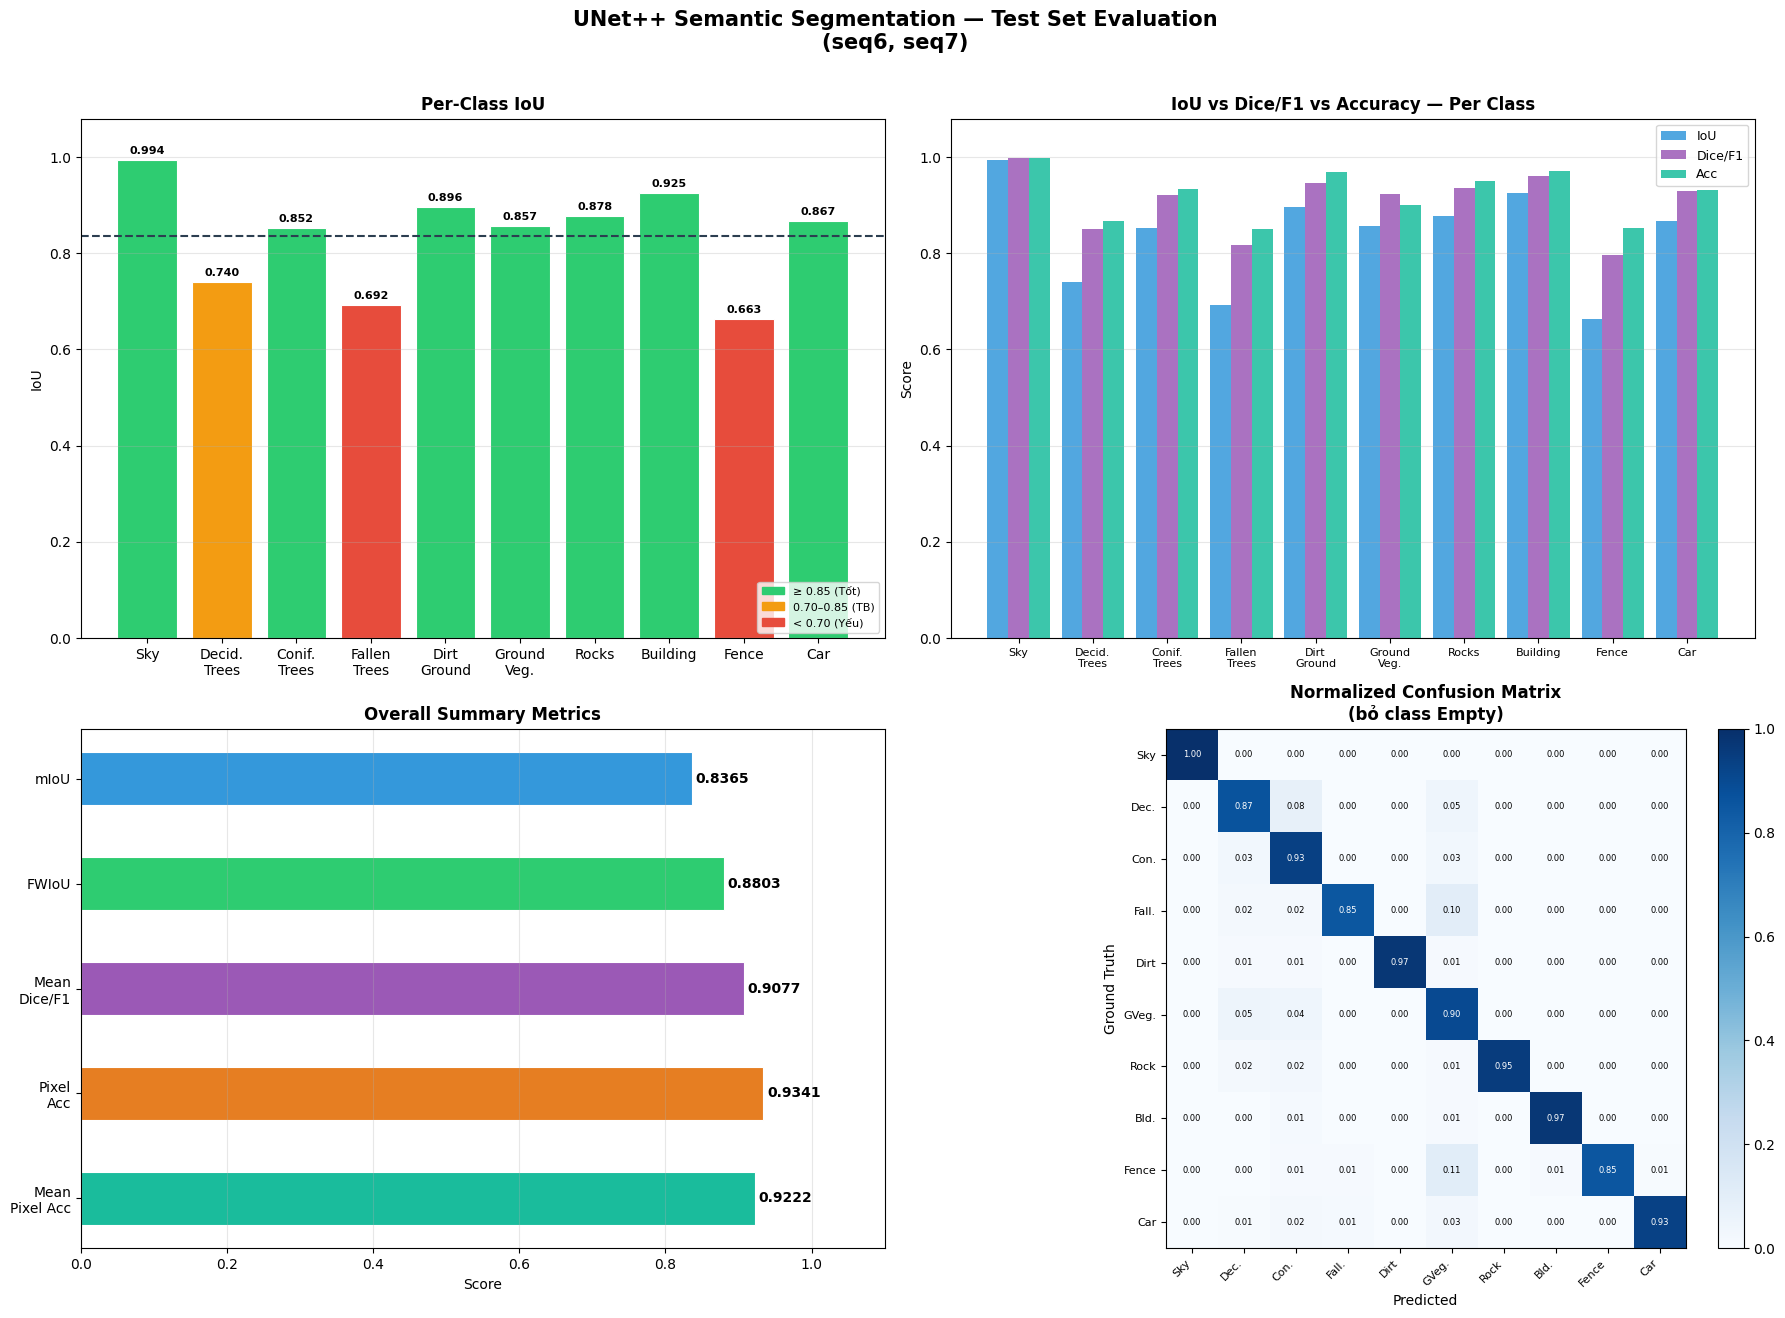
\includegraphics[width=\textwidth]{figures/fig_exp4_summary.png}
\caption{Tổng hợp đánh giá mô hình tốt nhất (Exp~4, adaptive) trên tập kiểm thử
(seq6, seq7): IoU theo lớp, so sánh IoU--Dice/F1--Accuracy, các chỉ số tổng thể
(mIoU $=0{,}8365$, FWIoU $=0{,}8803$, Pixel Acc $=0{,}9341$) và ma trận nhầm lẫn
chuẩn hóa.}
\label{fig:exp4_summary}
\end{figure}

\section{Kết quả theo từng lớp}
\label{sec:per_class}

Bảng~\ref{tab:perclass} là bằng chứng cốt lõi: IoU theo từng lớp cho thấy chính xác
chiến lược nào cải thiện lớp nào. Các lớp được sắp theo tần suất giảm dần; bốn lớp
hiếm ($<1\%$) được tô đậm.

\begin{table}[H]
\centering
\caption{IoU theo từng lớp trên tập kiểm thử (seq6, seq7).}
\label{tab:perclass}
\small
\begin{tabular}{l c c c c c}
\toprule
\textbf{Lớp} & \textbf{Tần suất} & \textbf{Exp1 CE} & \textbf{Exp2 CE+W} & \textbf{Exp3 FDC} & \textbf{Exp4 Adapt} \\
\midrule
Sky                & 20{,}33\% & 0{,}9940 & 0{,}9934 & 0{,}9936 & \textbf{0{,}9939} \\
Coniferous\_trees  & 27{,}85\% & \textbf{0{,}8550} & 0{,}8420 & 0{,}8454 & 0{,}8523 \\
Ground\_vegetation & 32{,}40\% & \textbf{0{,}8597} & 0{,}8475 & 0{,}8508 & 0{,}8570 \\
Deciduous\_trees   & 15{,}11\% & \textbf{0{,}7407} & 0{,}7235 & 0{,}7292 & 0{,}7404 \\
Dirt\_ground       & 1{,}83\%  & \textbf{0{,}8997} & 0{,}8890 & 0{,}8933 & 0{,}8959 \\
Rocks              & 1{,}74\%  & \textbf{0{,}8805} & 0{,}8634 & 0{,}8731 & 0{,}8782 \\
\textbf{Fallen\_trees} & \textbf{0{,}52\%} & 0{,}6706 & 0{,}6494 & 0{,}6711 & \textbf{0{,}6921} \\
\textbf{Building}  & \textbf{0{,}18\%}  & 0{,}9102 & 0{,}8729 & 0{,}9176 & \textbf{0{,}9252} \\
\textbf{Car}       & \textbf{0{,}04\%}  & 0{,}8232 & 0{,}8419 & 0{,}8545 & \textbf{0{,}8675} \\
\textbf{Fence}     & \textbf{0{,}01\%}  & 0{,}5535 & 0{,}6193 & 0{,}6413 & \textbf{0{,}6628} \\
\midrule
\textbf{mIoU}      &           & 0{,}8187 & 0{,}8142 & 0{,}8270 & \textbf{0{,}8365} \\
\bottomrule
\end{tabular}
\end{table}

\section{Phân tích trên các lớp hiếm}

Bảng~\ref{tab:rare} làm nổi bật mức cải thiện trên bốn lớp hiếm so với baseline.

\begin{table}[H]
\centering
\caption{Cải thiện IoU trên các lớp hiếm (so với Exp1, điểm phần trăm).}
\label{tab:rare}
\begin{tabular}{l c c c}
\toprule
\textbf{Lớp hiếm} & \textbf{Exp2 vs CE} & \textbf{Exp3 vs CE} & \textbf{Exp4 vs CE} \\
\midrule
Fence (0{,}01\%)        & $+6{,}58$ & $+8{,}78$ & \textbf{$+10{,}93$} \\
Car (0{,}04\%)          & $+1{,}87$ & $+3{,}13$ & \textbf{$+4{,}43$} \\
Building (0{,}18\%)     & $-3{,}73$ & $+0{,}74$ & \textbf{$+1{,}50$} \\
Fallen\_trees (0{,}52\%)& $-2{,}12$ & $+0{,}05$ & \textbf{$+2{,}15$} \\
\bottomrule
\end{tabular}
\end{table}

\noindent\textbf{Diễn giải:}
\begin{itemize}[leftmargin=1.4cm]
  \item \textbf{Exp 2 (CE+trọng số):} nâng được lớp cực hiếm (Fence $+6{,}6$,
  Car $+1{,}9$) nhưng \emph{làm hỏng} lớp Building ($-3{,}7$) và đa số các lớp phổ
  biến $\Rightarrow$ mIoU tổng giảm. Đây là dấu hiệu điển hình của over-weighting.
  \item \textbf{Exp 3 (Focal+Dice+CE):} cải thiện lớp hiếm mạnh hơn mà ít gây hại
  cho lớp phổ biến (nhờ Dice tối ưu vùng chồng lấp) $\Rightarrow$ mIoU tăng.
  \item \textbf{Exp 4 (thích nghi):} đạt mức cải thiện lớn nhất trên \emph{tất cả}
  lớp hiếm, đồng thời gần như khôi phục hiệu năng lớp phổ biến về mức baseline
  $\Rightarrow$ mIoU cao nhất. Trọng số học được giúp cân bằng tự động giữa các
  thành phần loss.
\end{itemize}

\begin{figure}[H]
\centering
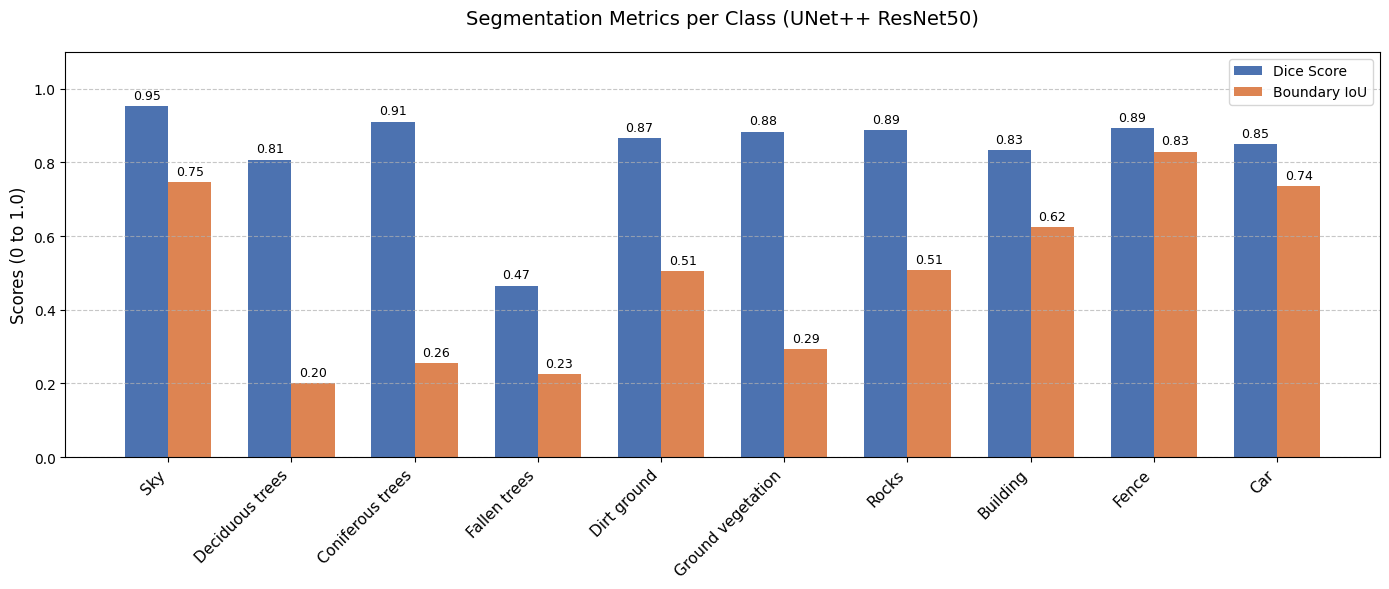
\includegraphics[width=\textwidth]{figures/fig_perclass_metrics.png}
\caption{Dice score và Boundary IoU theo từng lớp. Các lớp hiếm/nhỏ (Fallen trees,
Fence) có Boundary IoU thấp rõ rệt --- cho thấy khó khăn chủ yếu nằm ở vùng biên.}
\label{fig:perclass_metrics}
\end{figure}

\section{Diễn biến trọng số thích nghi (Exp 4)}

Trong Exp 4, ba trọng số $w_F, w_D, w_{CE}$ (suy ra từ $\sigma_k$ học được) thay đổi
theo epoch: khởi tạo $1{,}0$ và tăng dần trong các epoch đầu (ví dụ epoch~1:
$\approx 1{,}12/1{,}13/1{,}08$; epoch~3: $\approx 1{,}73/1{,}75/1{,}65$), cho thấy mô
hình tự điều chỉnh tỷ trọng giữa Focal, Dice và CE thay vì cố định thủ công. Giá trị
loss có thể âm do số hạng $\log\sigma_k$ (xem Mục~\ref{sec:adaptive}) --- hành vi
bình thường.

\HINH{Đường cong huấn luyện (loss \& mIoU) và diễn biến $w_F, w_D, w_{CE}$ theo epoch.}

\section{Kết quả định tính}

\begin{figure}[H]
\centering
\begin{subfigure}{0.48\textwidth}
  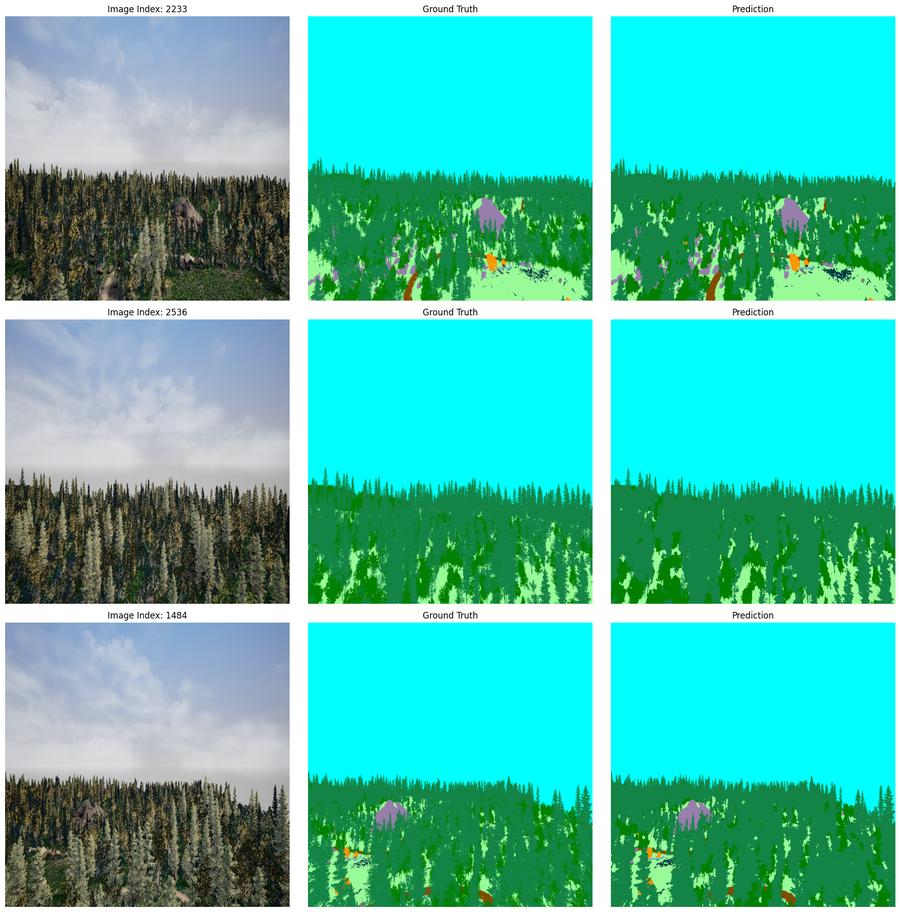
\includegraphics[width=\linewidth]{figures/qual_exp1.png}
  \caption{Exp 1 --- CE thuần}
\end{subfigure}\hfill
\begin{subfigure}{0.48\textwidth}
  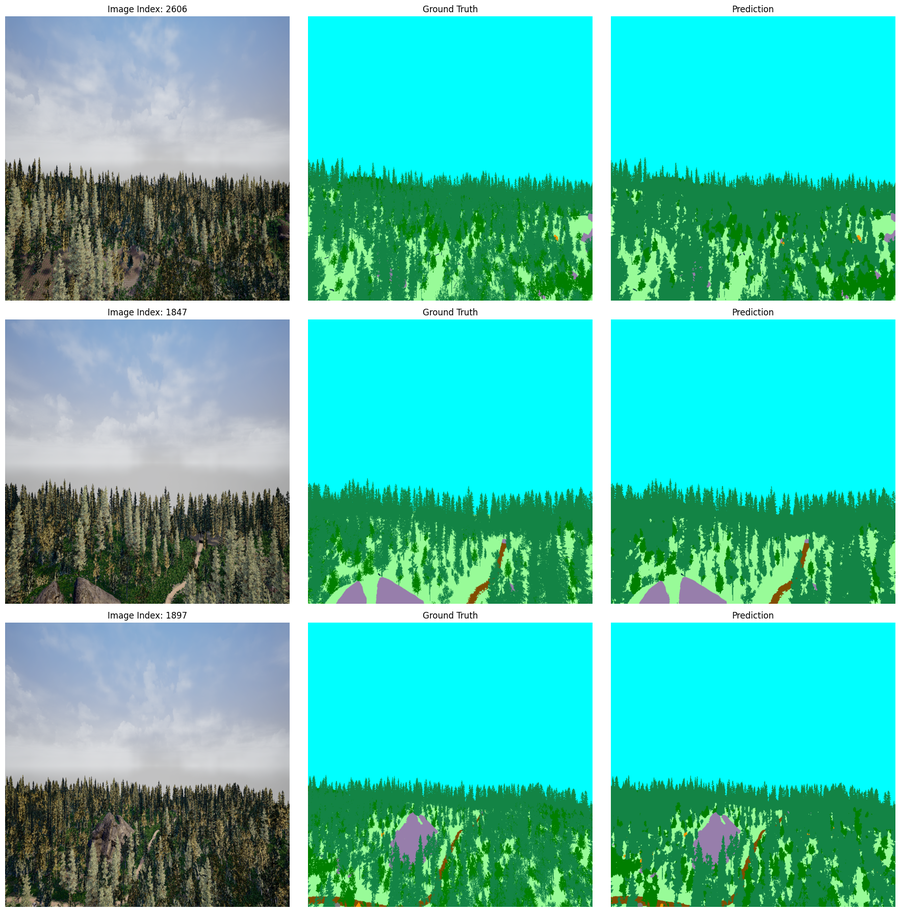
\includegraphics[width=\linewidth]{figures/qual_exp2.png}
  \caption{Exp 2 --- CE + trọng số}
\end{subfigure}

\vspace{4pt}
\begin{subfigure}{0.48\textwidth}
  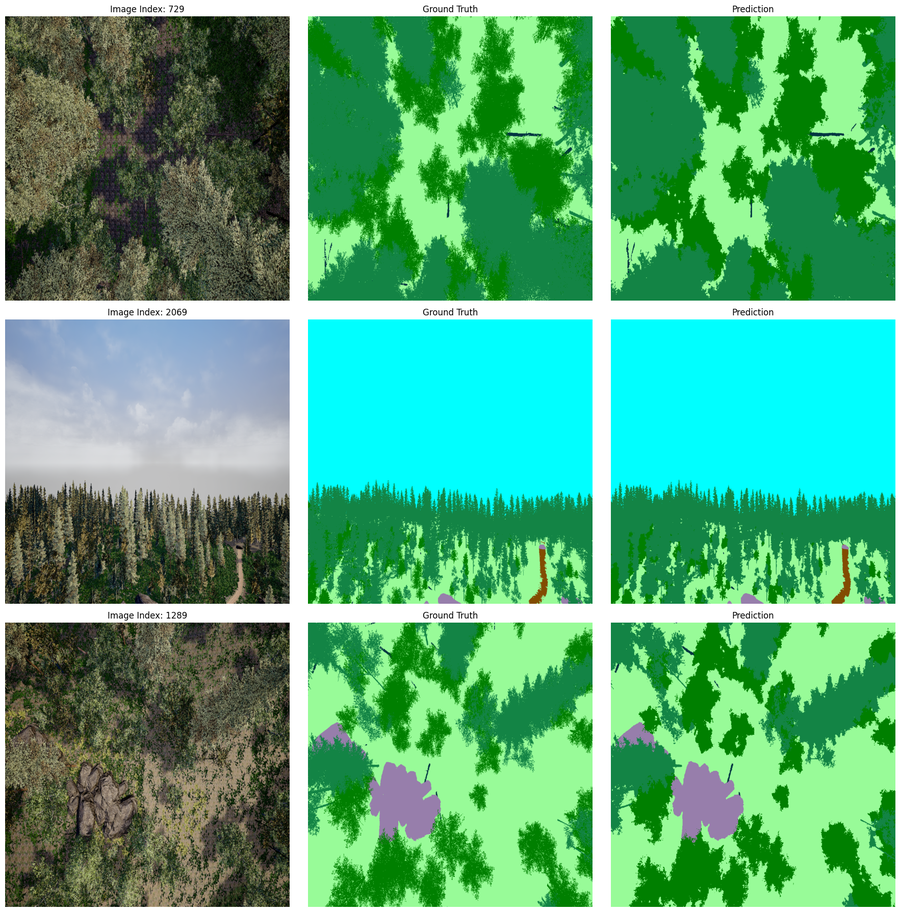
\includegraphics[width=\linewidth]{figures/qual_exp3.png}
  \caption{Exp 3 --- Focal+Dice+CE}
\end{subfigure}\hfill
\begin{subfigure}{0.48\textwidth}
  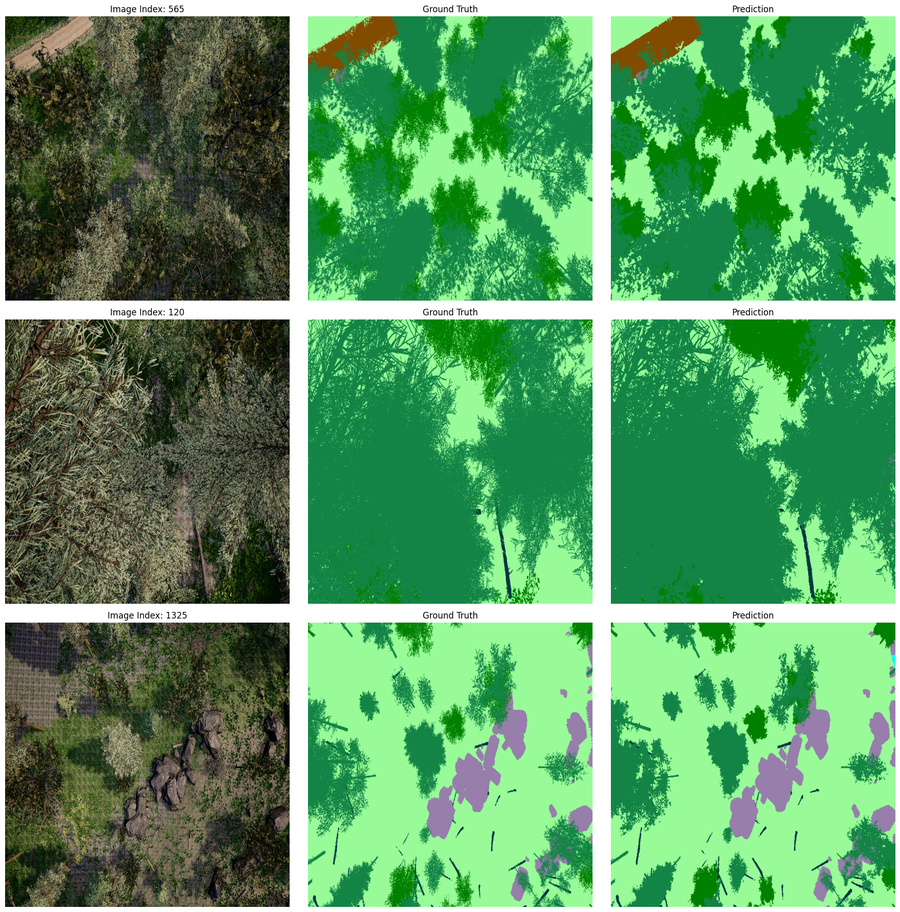
\includegraphics[width=\linewidth]{figures/qual_exp4.png}
  \caption{Exp 4 --- Adaptive}
\end{subfigure}
\caption{Kết quả định tính của bốn thí nghiệm trên tập kiểm thử (mỗi panel: 3 mẫu, cột
Ảnh gốc / Nhãn chuẩn / Dự đoán). \textit{Lưu ý:} các mẫu được chọn ngẫu nhiên độc lập
trong từng notebook nên không trùng nhau giữa các thí nghiệm.}
\label{fig:qual_montage}
\end{figure}

\TBD{Để so sánh trực tiếp công bằng: chạy lại inference của cả 4 mô hình trên CÙNG vài
chỉ số ảnh cố định, cắt cận cảnh vùng có Fence/Car, rồi thay hình ở trên.}

% =====================================================================
\section{Đánh giá độ bền theo điều kiện thời tiết \textnormal{(\TBD{đang tiến hành})}}
\label{sec:weather}

Để kiểm tra khả năng tổng quát hóa, mô hình tốt nhất (Exp 4) đang được đánh giá trên
các điều kiện ánh sáng/thời tiết khác nhau. Bảng~\ref{tab:weather} sẽ tổng hợp khi có
đủ kết quả.

\begin{table}[H]
\centering
\caption{mIoU theo điều kiện thời tiết (đánh giá chéo miền).}
\label{tab:weather}
\begin{tabular}{l c c c}
\toprule
\textbf{Điều kiện} & \textbf{Số ảnh} & \textbf{mIoU} & \textbf{Ghi chú} \\
\midrule
Sunny             & \TBD{} & \TBD{} & \TBD{} \\
Overcast          & \TBD{} & \TBD{} & \TBD{} \\
Sunny + Overcast  & \TBD{} & \TBD{} & \TBD{} \\
\bottomrule
\end{tabular}
\end{table}

\noindent\textit{Kết quả sơ bộ (một seed, chưa đầy đủ):} đánh giá chéo miền của mô
hình Exp 4 cho mIoU giảm đáng kể trên dữ liệu overcast ($\approx 0{,}55$) và dữ liệu
trộn ($\approx 0{,}59$--$0{,}72$), phản ánh domain gap về ánh sáng.
\TBD{Hoàn thiện và chuẩn hóa các phép đánh giá này; điền số chính thức vào bảng.}

% =====================================================================
\section{Đánh giá trên bộ dữ liệu WildUAV \textnormal{(\TBD{đang tiến hành})}}
\label{sec:wilduav}

Đánh giá trên bộ dữ liệu thực tế \textbf{WildUAV} nhằm kiểm tra khả năng chuyển miền
từ dữ liệu mô phỏng (AirSim) sang ảnh thực.

\begin{table}[H]
\centering
\caption{Kết quả trên WildUAV.}
\label{tab:wilduav}
\begin{tabular}{l c c c}
\toprule
\textbf{Mô hình / Loss} & \textbf{mIoU} & \textbf{PA} & \textbf{Ghi chú} \\
\midrule
Exp 4 (adaptive) & \TBD{} & \TBD{} & \TBD{ánh xạ lớp WildUAV $\leftrightarrow$ 11 lớp} \\
\bottomrule
\end{tabular}
\end{table}
\TBD{Bổ sung mô tả WildUAV (số ảnh, lớp, cách ánh xạ nhãn) và điền kết quả.}

% =====================================================================
\section{Mở rộng đa kiến trúc \textnormal{(\TBD{đang tiến hành})}}
\label{sec:multi_arch}

Ngoài UNet++/ResNet50, dự án hướng tới một \textbf{benchmark đa kiến trúc} (CNN,
Transformer, mô hình nhẹ) dùng hàm mất mát tốt nhất (adaptive), mỗi cấu hình chạy 3
seed để bảo đảm ý nghĩa thống kê. Bảng~\ref{tab:matrix} là ma trận thực nghiệm dự
kiến (25 cấu hình, chia 5 nhóm).

\begin{table}[H]
\centering
\caption{Ma trận thực nghiệm đa kiến trúc dự kiến (25 cấu hình $\times$ 3 seed).}
\label{tab:matrix}
\small
\begin{tabular}{c l l l}
\toprule
\textbf{Nhóm} & \textbf{Mục đích} & \textbf{Decoder} & \textbf{Encoder} \\
\midrule
A & CNN baseline      & UNet, DeepLabV3+, UNet++ & resnet34/50/101 \\
B & CNN hiện đại      & UNet, UPerNet, DeepLabV3+ & efficientnet, convnext, se\_resnet \\
C & Transformer       & SegFormer, UPerNet & mit\_b3/b5, swinv2, pvt\_v2 \\
D & Ablation decoder  & UNet/DLV3+/SegFormer/UPerNet/PSPNet/FPN & mit\_b3 (cố định) \\
E & HRNet \& nhẹ      & UNet, DeepLabV3+, Linknet & hrnet\_w48, mobilenet\_v2, mobileone \\
\bottomrule
\end{tabular}
\end{table}

Kết quả chính thức (cùng loss adaptive, cùng split, 3 seed) sẽ tổng hợp ở
Bảng~\ref{tab:multiarch}.

\begin{table}[H]
\centering
\caption{So sánh đa kiến trúc (cùng loss adaptive, cùng split, 3 seed).}
\label{tab:multiarch}
\small
\begin{tabular}{l l c c c c}
\toprule
\textbf{Decoder} & \textbf{Encoder} & \textbf{Test mIoU} & \textbf{Params} & \textbf{FLOPs} & \textbf{FPS} \\
\midrule
UNet++ & ResNet50 & 0{,}8365$^\dagger$ & 48{,}99M & 230{,}47G & 12{,}5 \\
\TBD{} & \TBD{} & \TBD{} & \TBD{} & \TBD{} & \TBD{} \\
\bottomrule
\end{tabular}
\end{table}
{\footnotesize $^\dagger$ một seed (2025), $1024\times1024$. Các dòng khác: \TBD{bổ sung}.}

\subsection*{Kết quả sơ bộ (split/cấu hình cũ --- chỉ để tham khảo)}
Trước nghiên cứu này, ba kiến trúc đã được đánh giá nhưng trên \textbf{split kiểm thử
khác} (seq9) và \textbf{cấu hình chưa đồng nhất} (kích thước ảnh, loss, patience khác
nhau), nên \textbf{không so sánh trực tiếp} được với các con số trong báo cáo:
SegFormer/MiT-B5 $\approx 0{,}703$; DeepLabV3+/MiT-B5 $\approx 0{,}683$;
UNet++/ResNet50 $\approx 0{,}605$. Các giá trị này gợi ý lợi thế của encoder
Transformer, và sẽ được chạy lại với cấu hình đồng nhất.
\TBD{Chạy lại 3 kiến trúc trên với loss adaptive + cùng split/cấu hình rồi điền vào
Bảng~\ref{tab:multiarch}.}

% =====================================================================
\section{Đánh giá nhiều seed (Exp 4) \textnormal{(\TBD{một phần})}}
\label{sec:multiseed}

Để đảm bảo ý nghĩa thống kê, Exp 4 cần chạy trên 3 seed. Hiện mới có seed 2025.

\begin{table}[H]
\centering
\caption{Exp 4 trên nhiều seed.}
\label{tab:seeds}
\begin{tabular}{c c}
\toprule
\textbf{Seed} & \textbf{Test mIoU} \\
\midrule
2025 & 0{,}8365 \\
42   & \TBD{} \\
123  & \TBD{} \\
\midrule
\textbf{Trung bình $\pm$ độ lệch} & \TBD{} \\
\bottomrule
\end{tabular}
\end{table}
\TBD{Chạy seed 42 và 123 cho Exp 4, điền giá trị và tính trung bình $\pm$ std.}
